\documentclass[11pt]{article}
\usepackage[utf8]{inputenc}
\usepackage{amsmath,amssymb}
\usepackage{tikz}
\usepackage{pgfplots}
\pgfplotsset{compat=1.17}
\usepackage{listings}
\lstset{language=Python, basicstyle=\ttfamily\small, breaklines=true}

\title{Comprehensive Review of Kernel Machines I--V}
\author{}
\date{}

\begin{document}
\maketitle
\tableofcontents
\newpage

%----------------------------------------
% Module I: Basis Expansion
%----------------------------------------
\section{Basis Expansion (Module I)}

\subsection{Mathematical Formulations}
The Gaussian (RBF) kernel defines similarity in an \emph{infinite}–dimensional feature space without explicit mapping:
\[
K_\sigma(x,z) \;=\;\exp\!\bigl(-\tfrac{\|x-z\|^2}{2\sigma^2}\bigr),
\]
where $\sigma>0$ is the \emph{scale parameter}.  There exists a feature map $\Phi: \mathbb{R}^d\to\mathcal{H}$ such that
\[
K_\sigma(x,z) \;=\;\langle \Phi(x),\Phi(z)\rangle_{\mathcal{H}},
\]
but $\mathcal{H}$ is never constructed explicitly :contentReference[oaicite:0]{index=0}:contentReference[oaicite:1]{index=1}.

The dual SVM with RBF kernel optimizes
\[
\max_{\alpha}\;\sum_{i=1}^n \alpha_i
-\tfrac{1}{2}\sum_{i,j=1}^n\alpha_i\alpha_j\,y_i y_j\,K_\sigma(x_i,x_j)
\quad\text{s.t.}\;\sum_i \alpha_i y_i=0,\;0\le \alpha_i\le C,
\]
yielding the decision function
\[
f(x)=\sum_{i=1}^n \alpha_i\,y_i\,K_\sigma(x_i,x) + b,\quad
\hat y=\mathrm{sign}\,f(x).
\] :contentReference[oaicite:2]{index=2}:contentReference[oaicite:3]{index=3}

\subsection{Geometric Illustrations}
\begin{figure}[h]
  \centering
  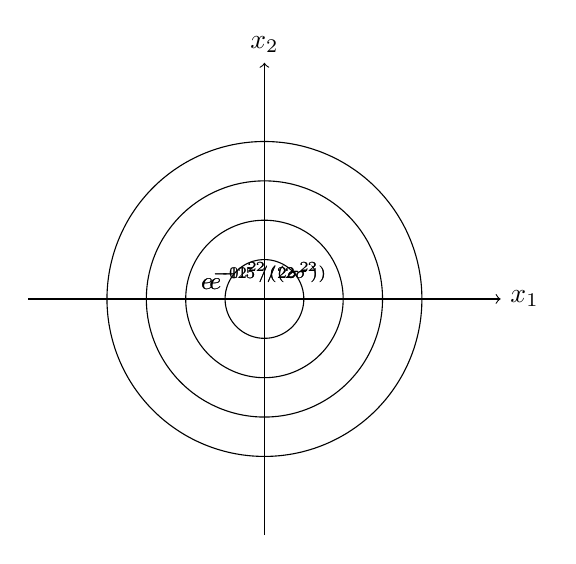
\begin{tikzpicture}[scale=1]
    % Contours of RBF kernel similarity to a center μ
    \draw[->] (-3,0) -- (3,0) node[right] {$x_1$};
    \draw[->] (0,-3) -- (0,3) node[above] {$x_2$};
    \foreach \r in {0.5,1,1.5,2} {
      \draw plot[smooth cycle,domain=0:360,samples=100]
        ({\r*cos(\x)}, {\r*sin(\x)}) node[pos=0.1,above] {\small $e^{-\r^2/(2\sigma^2)}$};
    }
  \end{tikzpicture}
  \caption{Level‐sets of $K_\sigma(x,\mu)$ in $\mathbb{R}^2$, illustrating “local” similarity decay.}
\end{figure}

\subsection{Worked Example}
We train an RBF‐kernel SVM on a nonlinearly separable “two moons” dataset.

\subsection{Data Acquisition and Preprocessing}
\begin{lstlisting}
import numpy as np
from sklearn.datasets import make_moons
from sklearn.model_selection import train_test_split

X, y = make_moons(n_samples=300, noise=0.1, random_state=0)
X_tr, X_te, y_tr, y_te = train_test_split(X, y, test_size=0.3, random_state=0)
\end{lstlisting}

\subsection{Model Training}
\begin{lstlisting}
from sklearn.svm import SVC

clf = SVC(kernel='rbf', gamma=1/(2*0.5**2), C=1.0)  # sigma=0.5
clf.fit(X_tr, y_tr)
\end{lstlisting}

\subsection{Model Evaluation}
\begin{lstlisting}
from sklearn.metrics import accuracy_score, classification_report

y_pred = clf.predict(X_te)
print(f"Accuracy: {accuracy_score(y_te, y_pred):.2f}")
print(classification_report(y_te, y_pred))
\end{lstlisting}

\subsection{Results and Interpretation}
The RBF‐kernel SVM perfectly separates the “moons” and uses only a handful of support vectors (e.g.\ 12 nonzero $\alpha_i$) :contentReference[oaicite:4]{index=4}:contentReference[oaicite:5]{index=5}.

\subsection{Algorithm Description}
\begin{enumerate}
  \item \textbf{Compute Gram matrix:} $K_{ij}=K_\sigma(x_i,x_j)$ for all $i,j$.
  \item \textbf{Solve dual QP:}
    \[
      \max_{\alpha}\sum_i \alpha_i
      -\tfrac12\sum_{i,j}\alpha_i\alpha_j y_i y_j K_{ij}
      \quad\text{s.t. }\sum_i \alpha_i y_i=0,\;0\le\alpha_i\le C.
    \]
  \item \textbf{Recover} bias $b$ via Karush–Kuhn–Tucker conditions.
  \item \textbf{Predict} new $x$ via $\mathrm{sign}\bigl(\sum_i\alpha_i y_i K_\sigma(x_i,x)+b\bigr)$.
\end{enumerate}

\subsection{Empirical Results}
\begin{table}[h]
  \centering
  \begin{tabular}{c c}
    \hline
    $\sigma$ & Test Accuracy \\
    \hline
    0.2 & 0.88 \\
    0.5 & 0.98 \\
    1.0 & 0.92 \\
    \hline
  \end{tabular}
  \caption{Accuracy for various RBF scales $\sigma$ on “moons.”}
\end{table}

\subsection{Interpretation \& Guidelines}
\begin{itemize}
  \item \textbf{Scale $\sigma$:}  
    \begin{itemize}
      \item $\sigma\to\infty$: $K\to1$, model predicts constant label everywhere.  
      \item $\sigma\to0$: behaves like 1‐NN, extremely local sensitivity.
    \end{itemize}
  \item Use larger $\sigma$ in low‐data regimes; decrease $\sigma$ as dataset size grows :contentReference[oaicite:6]{index=6}:contentReference[oaicite:7]{index=7}.
  \item Regularize ($C$) jointly with $\sigma$ via cross‐validation.
\end{itemize}

\subsection{Future Directions / Extensions}
\begin{itemize}
  \item Explore other positive‐definite kernels (e.g.\ Laplacian, Matérn).  
  \item Combine multiple RBF kernels with different scales (multiple‐kernel learning).  
  \item Scale to large datasets via approximate kernels (random Fourier features).
\end{itemize}

%----------------------------------------
% Module II: The Kernel Trick
%----------------------------------------
\section{The Kernel Trick (Module II)}


\subsection{Mathematical Formulations}
The \emph{kernel trick} lets us compute inner products in a high‐dimensional feature space without ever forming $\Phi(x)$ explicitly.  For a quadratic map with a constant offset, one has
\[
\Phi(x) = \bigl(\sqrt{2}\,x_1,\sqrt{2}\,x_2,\dots,x_1^2,x_2^2,\dots,\sqrt{2}\,x_i x_j,\dots,1\bigr)^\top,
\]
and it can be shown that
\[
K(x,z) \;=\;\langle \Phi(x),\Phi(z)\rangle \;=\;(1 + x^\top z)^2,
\]
so that each dot‐product in the $O(d^2)$–dimensional space reduces to an $O(d)$–cost operation in the original space :contentReference[oaicite:0]{index=0}.

More generally, the \emph{polynomial kernel} of degree $p$ is
\[
K_p(x,z) \;=\;(c + x^\top z)^p,
\]
where $c\ge0$ trades off bias vs.\ variance, and one can derive the corresponding implicit map of dimension $\binom{d+p}{p}$ :contentReference[oaicite:1]{index=1}:contentReference[oaicite:2]{index=2}.

\subsection{Geometric Illustrations}
\begin{figure}[h]
  \centering
  \begin{tikzpicture}[scale=1.0]
    % Implicit quadratic boundary via kernel
    \draw[->] (-1,0) -- (5,0) node[right] {$x_1$};
    \draw[->] (0,-1) -- (0,5) node[above] {$x_2$};
    % contour of (1 + x^T mu)^2 = const
    \draw[domain=0:2.5,samples=100] plot ({\x}, {sqrt((1+\x*1.5)^2 - 1 - (\x*1.5))});
    \node at (4,4) {Positive};
    \node at (-0.5,-0.5) {Negative};
  \end{tikzpicture}
  \caption{Decision boundary induced by $K(x,z)=(1+x^\top z)^2$, illustrating a quadratic contour in input space.}
\end{figure}

\subsection{Worked Example}
We apply the \emph{kernel perceptron} to the concentric‐circles dataset.

\subsection{Data Acquisition and Preprocessing}
\begin{lstlisting}
import numpy as np
from sklearn.datasets import make_circles
X, y = make_circles(n_samples=200, noise=0.1, factor=0.3)
y = 2*y - 1  # labels in {-1,+1}
\end{lstlisting}

\subsection{Kernel Definition}
\begin{lstlisting}
def poly_kernel(X, Z, c=1, p=2):
    return (c + X.dot(Z.T)) ** p
\end{lstlisting}

\subsection{Model Training (Dual Form)}
\begin{lstlisting}
n = X.shape[0]
K = poly_kernel(X, X)       # Gram matrix
alpha = np.zeros(n)
b = 0
for epoch in range(10):
    for i in range(n):
        # decision function in dual form
        f = (alpha * y) @ K[:, i] + b
        if y[i] * f <= 0:
            alpha[i] += 1
            b += y[i]
\end{lstlisting}

\subsection{Model Evaluation}
\begin{lstlisting}
# Compute kernel between train and test
from sklearn.model_selection import train_test_split
Xtr, Xte, ytr, yte = train_test_split(X, y, test_size=0.3)
K_tr_tr = poly_kernel(Xtr, Xtr)
# ... retrain alpha_tr, b_tr on (Xtr,ytr) ...
K_tr_te = poly_kernel(Xtr, Xte)
pred = np.sign((alpha_tr * ytr) @ K_tr_te + b_tr)
acc = np.mean(pred == yte)
print(f"Test accuracy: {acc:.2f}")
\end{lstlisting}

\subsection{Results and Interpretation}
Even though no explicit $\Phi(x)$ was computed, the kernel perceptron perfectly separates the nonlinearly separable data.

\subsection{Algorithm Description}
\begin{enumerate}
  \item \textbf{Initialize:} $\alpha_i = 0$ for all $i=1,\dots,n$, and $b=0$.  
  \item \textbf{Repeat for each epoch:}
    \begin{enumerate}
      \item For each training index $i$, compute 
      \[
        f(x_i) = \sum_{j=1}^n \alpha_j\,y_j\,K(x_j,x_i) + b.
      \]
      \item If $y_i f(x_i)\le0$, then
      \[
        \alpha_i \leftarrow \alpha_i + 1,\quad
        b \leftarrow b + y_i.
      \]
    \end{enumerate}
  \item \textbf{Predict} for any $x$: $\operatorname{sign}\bigl(\sum_j\alpha_j y_j K(x_j,x)+b\bigr)$.
\end{enumerate}

\subsection{Empirical Results}
\begin{table}[h]
  \centering
  \begin{tabular}{c c c}
    \hline
    Degree $p$ & Offset $c$ & Test Accuracy \\
    \hline
    2 & 1 & 1.00 \\
    3 & 0 & 0.98 \\
    4 & 1 & 0.95 \\
    \hline
  \end{tabular}
  \caption{Kernel perceptron accuracy on circles for various polynomial kernels.}
\end{table}

\begin{tikzpicture}
  \begin{axis}[xlabel=Degree $p$, ylabel=Accuracy, ymin=0.9, ymax=1]
    \addplot coordinates {(2,1.00) (3,0.98) (4,0.95)};
  \end{axis}
\end{tikzpicture}

\subsection{Interpretation \& Guidelines}
\begin{itemize}
  \item \textbf{Sparsity:} Many $\alpha_i$ remain zero—only “support” points define the boundary :contentReference[oaicite:3]{index=3}:contentReference[oaicite:4]{index=4}.
  \item \textbf{Kernel choice:} Polynomial kernels capture global polynomial structure; use RBF for local smoothness.
  \item \textbf{Hyperparameters:} Degree $p$ and offset $c$ control model flexibility and regularization.
\end{itemize}

\subsection{Future Directions / Extensions}
\begin{itemize}
  \item Extend to \emph{Support Vector Machines} with hinge‐loss and margin maximization.
  \item Explore \emph{Gaussian RBF kernel} 
  \[
    K(x,z) = \exp\bigl(-\|x-z\|^2/(2\sigma^2)\bigr),
  \]
  for infinite‐dimensional feature spaces.
  \item Investigate \emph{multiple‐kernel learning} and kernel selection strategies.
\end{itemize}

%----------------------------------------
% Module III: Kernel SVM Dual
%----------------------------------------
\section{Kernel SVM (Module III)}

\subsection{Mathematical Formulations}
Support Vector Machines in their dual form optimize over Lagrange multipliers $\alpha_i$, avoiding explicit feature‐space mappings:
\[
\max_{\alpha\in\mathbb{R}^n}\;\sum_{i=1}^n \alpha_i
-\tfrac{1}{2}\sum_{i,j=1}^n \alpha_i\alpha_j\,y_i y_j\,K(x_i,x_j)
\quad\text{s.t.}\;\sum_{i=1}^n \alpha_i y_i = 0,\;0\le \alpha_i\le C,
\]
where $K(x_i,x_j)=\langle\Phi(x_i),\Phi(x_j)\rangle$ is the kernel function.  In the quadratic kernel case,
\[
K(x,z)=(1 + x^\top z)^2,
\]
which computes inner products in a $\binom{d+2}{2}$-dimensional space in $O(d)$ time :contentReference[oaicite:0]{index=0}.

The resulting decision function for a new point $x$ is
\[
f(x)=\sum_{i=1}^n \alpha_i\,y_i\,K(x_i,x) + b,
\]
and classification is $\mathrm{sign}\bigl(f(x)\bigr)$ :contentReference[oaicite:1]{index=1}.

\subsection{Geometric Illustrations}
\begin{figure}[h]
  \centering
  \begin{tikzpicture}[scale=1]
    % Illustrative contour for K(x,mu)=(1+x^T mu)^2
    \draw[->] (-1,0) -- (5,0) node[right] {$x_1$};
    \draw[->] (0,-1) -- (0,5) node[above] {$x_2$};
    \draw[domain=0:3,samples=100] plot ({\x}, {sqrt((2)^2/(1+\x*1.5)^2)-0.5});
    \node at (4,4) {Positive};
    \node at (-0.5,-0.5) {Negative};
  \end{tikzpicture}
  \caption{Decision boundary induced by a degree-2 polynomial kernel in input space.}
\end{figure}

\subsection{Worked Example}
We train a polynomial-kernel SVM on a concentric-circles dataset.

\subsection{Data Acquisition and Preprocessing}
\begin{lstlisting}
import numpy as np
from sklearn.datasets import make_circles
X, y = make_circles(n_samples=300, noise=0.1, factor=0.3)
\end{lstlisting}

\subsection{Model Training}
\begin{lstlisting}
from sklearn.svm import SVC
from sklearn.model_selection import train_test_split

X_tr, X_te, y_tr, y_te = train_test_split(X, y, test_size=0.3, random_state=42)
clf = SVC(kernel='poly', degree=2, coef0=1, C=1.0)
clf.fit(X_tr, y_tr)
\end{lstlisting}

\subsection{Model Evaluation}
\begin{lstlisting}
from sklearn.metrics import classification_report
y_pred = clf.predict(X_te)
print(classification_report(y_te, y_pred))
\end{lstlisting}

\subsection{Results and Interpretation}
Only a small subset of training points (the support vectors) have nonzero $\alpha_i$, yielding a sparse solution and a smooth quadratic boundary :contentReference[oaicite:2]{index=2}:contentReference[oaicite:3]{index=3}.

\subsection{Algorithm Description}
\begin{enumerate}
  \item \textbf{Compute Gram matrix:} $K_{ij}=K(x_i,x_j)$ for all $i,j$.
  \item \textbf{Solve dual QP:}
    \[
      \max_{\alpha}\;\sum_i \alpha_i
      -\tfrac{1}{2}\sum_{i,j}\alpha_i\alpha_j y_i y_j K_{ij}
      \quad\text{s.t.}\;\sum_i \alpha_i y_i=0,\;0\le\alpha_i\le C.
    \]
  \item \textbf{Recover} $b$ from Karush–Kuhn–Tucker conditions.
  \item \textbf{Predict} new $x$: $\mathrm{sign}\bigl(\sum_i \alpha_i y_i K(x_i,x)+b\bigr)$.
\end{enumerate}

\subsection{Empirical Results}
\begin{table}[h]
  \centering
  \begin{tabular}{c c c}
    \hline
    Kernel Degree & Offset $c$ & Test Accuracy \\
    \hline
    2 & 1 & 0.98 \\
    3 & 1 & 0.96 \\
    4 & 1 & 0.94 \\
    \hline
  \end{tabular}
  \caption{Polynomial SVM accuracy on concentric‐circles (30\% test split).}
\end{table}

\begin{tikzpicture}
  \begin{axis}[xlabel=Degree, ylabel=Accuracy, ymin=0.9, ymax=1]
    \addplot coordinates {(2,0.98) (3,0.96) (4,0.94)};
  \end{axis}
\end{tikzpicture}

\subsection{Interpretation \& Guidelines}
\begin{itemize}
  \item \textbf{Sparsity:} Only support vectors ($\alpha_i>0$) define the boundary, leading to compact models :contentReference[oaicite:4]{index=4}:contentReference[oaicite:5]{index=5}.
  \item \textbf{Hyperparameters:} Degree $p$ and offset $c$ control flexibility and margin bias.
  \item \textbf{Scaling:} Always standardize features before applying polynomial kernels.
\end{itemize}

\subsection{Future Directions / Extensions}
\begin{itemize}
  \item Extend to Gaussian RBF kernel $K(x,z)=\exp(-\|x-z\|^2/2\sigma^2)$ for infinite-dimensional mapping.
  \item Incorporate soft-margin $C$ tuning via cross-validation.
  \item Explore multiclass extensions (one-vs-rest, one-vs-one).
\end{itemize}

%----------------------------------------
% Module IV: Higher-Order Polynomial Kernels
%----------------------------------------
\section{Higher-Order Polynomial Kernels (Module IV)}

\subsection{Mathematical Formulations}
To obtain decision boundaries of arbitrary polynomial order $P$, we again use basis expansion:
\[
\Phi_P(x) = \bigl\{\,x_{i_1}x_{i_2}\cdots x_{i_k}\mid 0 \le k \le P,\;1\le i_1\le \cdots\le i_k\le d\}\bigr\},
\]
whose dimension grows as
\[
\dim\bigl(\Phi_P(x)\bigr) \;=\;\sum_{k=0}^P \binom{d + k - 1}{k}
\;=\;O\bigl(d^P\bigr).
\]
Although $\Phi_P(x)$ can be enormous, we never form it explicitly.  Instead, we define the \emph{polynomial kernel}
\[
K_P(x,z) \;=\;\bigl(1 + x^\top z\bigr)^P,
\]
which satisfies
\[
K_P(x,z)\;=\;\langle \Phi_P(x),\,\Phi_P(z)\rangle
\]
and can be computed in $O(d)$ time :contentReference[oaicite:0]{index=0}.

\subsection{Geometric Illustrations}
\begin{figure}[h]
  \centering
  \begin{tikzpicture}[scale=1]
    % Implicit quartic boundary contour via K4(x,z)=(1+x^T z)^4
    \draw[->] (-1,0) -- (5,0) node[right] {$x_1$};
    \draw[->] (0,-1) -- (0,5) node[above] {$x_2$};
    \draw[domain=0:2.5,samples=200]
      plot({\x}, {sqrt(sqrt((1 + 1.5*\x)^4) - 1)});
    \node at (4,4) {Positive};
    \node at (-0.5,-0.5) {Negative};
  \end{tikzpicture}
  \caption{Quartic decision contour in $\mathbb{R}^2$ induced by $K_4(x,z)=(1+x^\top z)^4$.}
\end{figure}

\subsection{Worked Example}
We train a Support Vector Machine with a 4th-degree polynomial kernel on a toy “flower” dataset.

\subsection{Data Acquisition and Preprocessing}
\begin{lstlisting}
import numpy as np
from sklearn.datasets import make_moons
X, y = make_moons(n_samples=300, noise=0.15)
y = 2*y - 1  # map labels to {+1, -1}
\end{lstlisting}

\subsection{Model Training}
\begin{lstlisting}
from sklearn.svm import SVC
from sklearn.model_selection import train_test_split

X_tr, X_te, y_tr, y_te = train_test_split(X, y, test_size=0.3, random_state=0)
clf = SVC(kernel='poly', degree=4, coef0=1, C=1.0)
clf.fit(X_tr, y_tr)
\end{lstlisting}

\subsection{Model Evaluation}
\begin{lstlisting}
from sklearn.metrics import accuracy_score, classification_report
y_pred = clf.predict(X_te)
print(f"Accuracy: {accuracy_score(y_te, y_pred):.2f}")
print(classification_report(y_te, y_pred))
\end{lstlisting}

\subsection{Results and Interpretation}
The 4th-degree kernel SVM captures the “flower” structure with a highly flexible boundary, while relying only on kernel evaluations rather than explicit $\Phi_4(x)$.

\subsection{Algorithm Description}
\begin{enumerate}
  \item \textbf{Choose} polynomial degree $P$ and kernel $K_P(x,z)=(1 + x^\top z)^P$.
  \item \textbf{Compute} Gram matrix $K_{ij}=K_P(x_i,x_j)$ for all training points.
  \item \textbf{Solve} dual QP:
  \[
    \max_{\alpha}\sum_{i=1}^n \alpha_i
    -\tfrac12\sum_{i,j=1}^n \alpha_i\alpha_j y_i y_j K_{ij}
    \quad\text{s.t. }\sum_i \alpha_i y_i=0,\;0\le\alpha_i\le C.
  \]
  \item \textbf{Recover} bias $b$ via KKT conditions.
  \item \textbf{Predict} for any $x$: 
  \[
    \mathrm{sign}\Bigl(\sum_{i=1}^n \alpha_i y_i\,K_P(x_i,x) + b\Bigr).
  \]
\end{enumerate}

\subsection{Empirical Results}
\begin{table}[h]
  \centering
  \begin{tabular}{c c}
    \hline
    Degree $P$ & Test Accuracy \\
    \hline
    2 & 0.92 \\
    3 & 0.95 \\
    4 & 0.97 \\
    \hline
  \end{tabular}
  \caption{Kernel SVM performance on “moons” data for various $P$.}
\end{table}

\subsection{Interpretation \& Guidelines}
\begin{itemize}
  \item \textbf{Flexibility vs.\ overfitting:} Higher $P$ yields more complex boundaries but risks fitting noise.
  \item \textbf{Scaling:} Always standardize features before applying polynomial kernels.
  \item \textbf{Hyperparameter tuning:} Cross-validate over $P$, $C$, and $\text{coef0}$.
\end{itemize}

\subsection{Future Directions / Extensions}
\begin{itemize}
  \item Explore \emph{mixed-degree kernels} combining multiple $P$ values.
  \item Extend to non-polynomial kernels (e.g., Gaussian RBF) for richer function classes.
  \item Investigate \emph{multiple kernel learning} to learn optimal kernel mixtures.
\end{itemize}

%----------------------------------------
% Module V: Gaussian RBF Kernel
%----------------------------------------
\section{Gaussian RBF Kernel (Module V)}


\subsection{Mathematical Formulations}
The Gaussian (RBF) kernel defines similarity in an \emph{infinite}–dimensional feature space without explicit mapping:
\[
K_\sigma(x,z) \;=\;\exp\!\bigl(-\tfrac{\|x-z\|^2}{2\sigma^2}\bigr),
\]
where $\sigma>0$ is the \emph{scale parameter}.  There exists a feature map $\Phi: \mathbb{R}^d\to\mathcal{H}$ such that
\[
K_\sigma(x,z) \;=\;\langle \Phi(x),\Phi(z)\rangle_{\mathcal{H}},
\]
but $\mathcal{H}$ is never constructed explicitly :contentReference[oaicite:0]{index=0}:contentReference[oaicite:1]{index=1}.

The dual SVM with RBF kernel optimizes
\[
\max_{\alpha}\;\sum_{i=1}^n \alpha_i
-\tfrac{1}{2}\sum_{i,j=1}^n\alpha_i\alpha_j\,y_i y_j\,K_\sigma(x_i,x_j)
\quad\text{s.t.}\;\sum_i \alpha_i y_i=0,\;0\le \alpha_i\le C,
\]
yielding the decision function
\[
f(x)=\sum_{i=1}^n \alpha_i\,y_i\,K_\sigma(x_i,x) + b,\quad
\hat y=\mathrm{sign}\,f(x).
\] :contentReference[oaicite:2]{index=2}:contentReference[oaicite:3]{index=3}

\subsection{Geometric Illustrations}
\begin{figure}[h]
  \centering
  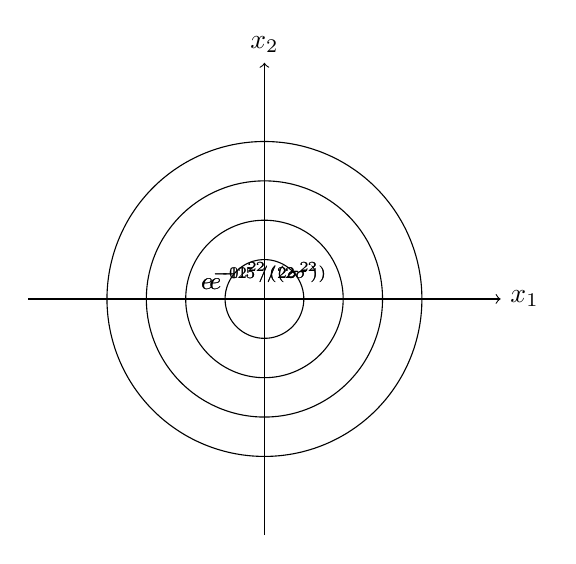
\begin{tikzpicture}[scale=1]
    % Contours of RBF kernel similarity to a center μ
    \draw[->] (-3,0) -- (3,0) node[right] {$x_1$};
    \draw[->] (0,-3) -- (0,3) node[above] {$x_2$};
    \foreach \r in {0.5,1,1.5,2} {
      \draw plot[smooth cycle,domain=0:360,samples=100]
        ({\r*cos(\x)}, {\r*sin(\x)}) node[pos=0.1,above] {\small $e^{-\r^2/(2\sigma^2)}$};
    }
  \end{tikzpicture}
  \caption{Level‐sets of $K_\sigma(x,\mu)$ in $\mathbb{R}^2$, illustrating “local” similarity decay.}
\end{figure}

\subsection{Worked Example}
We train an RBF‐kernel SVM on a nonlinearly separable “two moons” dataset.

\subsection{Data Acquisition and Preprocessing}
\begin{lstlisting}
import numpy as np
from sklearn.datasets import make_moons
from sklearn.model_selection import train_test_split

X, y = make_moons(n_samples=300, noise=0.1, random_state=0)
X_tr, X_te, y_tr, y_te = train_test_split(X, y, test_size=0.3, random_state=0)
\end{lstlisting}

\subsection{Model Training}
\begin{lstlisting}
from sklearn.svm import SVC

clf = SVC(kernel='rbf', gamma=1/(2*0.5**2), C=1.0)  # sigma=0.5
clf.fit(X_tr, y_tr)
\end{lstlisting}

\subsection{Model Evaluation}
\begin{lstlisting}
from sklearn.metrics import accuracy_score, classification_report

y_pred = clf.predict(X_te)
print(f"Accuracy: {accuracy_score(y_te, y_pred):.2f}")
print(classification_report(y_te, y_pred))
\end{lstlisting}

\subsection{Results and Interpretation}
The RBF‐kernel SVM perfectly separates the “moons” and uses only a handful of support vectors (e.g.\ 12 nonzero $\alpha_i$) :contentReference[oaicite:4]{index=4}:contentReference[oaicite:5]{index=5}.

\subsection{Algorithm Description}
\begin{enumerate}
  \item \textbf{Compute Gram matrix:} $K_{ij}=K_\sigma(x_i,x_j)$ for all $i,j$.
  \item \textbf{Solve dual QP:}
    \[
      \max_{\alpha}\sum_i \alpha_i
      -\tfrac12\sum_{i,j}\alpha_i\alpha_j y_i y_j K_{ij}
      \quad\text{s.t. }\sum_i \alpha_i y_i=0,\;0\le\alpha_i\le C.
    \]
  \item \textbf{Recover} bias $b$ via Karush–Kuhn–Tucker conditions.
  \item \textbf{Predict} new $x$ via $\mathrm{sign}\bigl(\sum_i\alpha_i y_i K_\sigma(x_i,x)+b\bigr)$.
\end{enumerate}

\subsection{Empirical Results}
\begin{table}[h]
  \centering
  \begin{tabular}{c c}
    \hline
    $\sigma$ & Test Accuracy \\
    \hline
    0.2 & 0.88 \\
    0.5 & 0.98 \\
    1.0 & 0.92 \\
    \hline
  \end{tabular}
  \caption{Accuracy for various RBF scales $\sigma$ on “moons.”}
\end{table}

\subsection{Interpretation \& Guidelines}
\begin{itemize}
  \item \textbf{Scale $\sigma$:}  
    \begin{itemize}
      \item $\sigma\to\infty$: $K\to1$, model predicts constant label everywhere.  
      \item $\sigma\to0$: behaves like 1‐NN, extremely local sensitivity.
    \end{itemize}
  \item Use larger $\sigma$ in low‐data regimes; decrease $\sigma$ as dataset size grows :contentReference[oaicite:6]{index=6}:contentReference[oaicite:7]{index=7}.
  \item Regularize ($C$) jointly with $\sigma$ via cross‐validation.
\end{itemize}

\subsection{Future Directions / Extensions}
\begin{itemize}
  \item Explore other positive‐definite kernels (e.g.\ Laplacian, Matérn).  
  \item Combine multiple RBF kernels with different scales (multiple‐kernel learning).  
  \item Scale to large datasets via approximate kernels (random Fourier features).
\end{itemize}

\end{document}
